\documentclass[../discrete.tex]{subfiles}
\graphicspath{{\subfix{../figures/}}}
\begin{document}
\chapter{Logic and Proofs}
\section{Propositional Logic}
A proposition is a declarative statement that is either true or false, but not both. We use letters to denote propositional variables. The conventional letters for propositional variables are $p,q,r,s$. True is notated as T and false is notated as F. An atomic proposition is a proposition that cannot be expressed in terms of simpler propositions.
\begin{definition}
    Let $p$ be a proposition. The negation of $p$, denoted by $\neg{p}$ (or $\bar{p}$) means "It is not the case that $p$".
    \smallbreak
    The proposition $\neg{p}$ is read as "not $p$". The truth value of the negation of $p$, $\neg{p}$ is the opposite of the truth value of $p$.
\end{definition}
The negation of a proposition can also be considered the result of the operation of the negation operator on a proposition. 

The next operator is a connective and it is used to form new propositions from two or more existing propositions.
\begin{definition}
    Let $p$ and $q$ be propositions. The conjunction of $p$ and $q$, denoted by $p\land q$, is the proposition of "$p$ and $q$". The conjunction $p\land q$ is true when both are true, and false when both are false.
\end{definition}
\begin{definition}
    Let $p$ and $q$ be propositions. The disjunction of $p$ and $q$, denoted by $p\lor q$, is the proposition "$p$ or $q$". The disjunction $p\lor q$ is false when both $p$ and $q$ are false, otherwise it is true.
\end{definition}
\begin{definition}
    Let $p$ and $q$ be propositions. The exclusive or of $p$ and $q$, denoted by $p\oplus{q}$ is the proposition that is true when exactly one of $p$ and $q$ is true and is false otherwise.
\end{definition}
There are other ways propositions can be combined.
\begin{definition}
    Let $p$ and $q$ be propositions. The conditional statement $p\rightarrow q$, is the proposition, "if $p$, then $q$". The conditional statement $p\rightarrow q$ is false when $p$ is true and $q$ is false, and true otherwise. $p$ is called the hypothesis and $q$ is called the conclusion.
\end{definition}
A conditional statement is also called an implication.

With $p\rightarrow q$, we can form three related conditional statements. 

The first is the proposition $q\rightarrow p$, which is the converse of $p\rightarrow q$. 

The contrapositive of $p\rightarrow q$ is $\neg q\rightarrow \neg p$.

The inverse of $p\rightarrow q$ is $\neg p \rightarrow \neg q$.

The contrapositive of a conditional statement is equal to it. We all two compound propositions equivalent when they always have the same truth values. The converse and inverse of a conditional statement are equivalent as well.

There is another way to combine propositions that expresses that two propositions have the same truth value.
\begin{definition}
    Let $p$ and $q$ be propositions. The biconditional statement $p\leftrightarrow q$ is the proposition "$p$ if and only $q$". This statement is true if $p$ and $q$ have the same truth values, and is false otherwise.
\end{definition}
The negation operator is applied before all logical operators. Another general rule is that the conjunction operator takes precendence over the disjunction operator. It is an accepted rule that conditional and biconditional operators have lower precendence than the conjuction and disjunction operators. 

A bit is a symbol with two values, 0 and 1. 1 is true, and 0 is false. 
\section{Propositional Equivalences}
\begin{definition}
    A compound proposition that is always true, no matter what the truth values of the propositional values that occur in it, is called a tautology. A compound proposition that is always false is called a contradiction. If it is neither a tautology or a contradiction, it is called a contingency.
\end{definition}
Compound propositions that have the same truth values in all possible cases are called logically equivalent. 
\begin{definition}
    The compound propositions $p$ and $q$ are called logically equivalent if $p\leftrightarrow q$ is a tautology. The notation $p\equiv q$ denotes that $p$ and $q$ are logically equivalent.
\end{definition}
We can establish logical equivalence of more than two compound propositions. Generally $2^n$ rows are required if a compound proposition involves $n$ propositional variables.
\begin{center}
    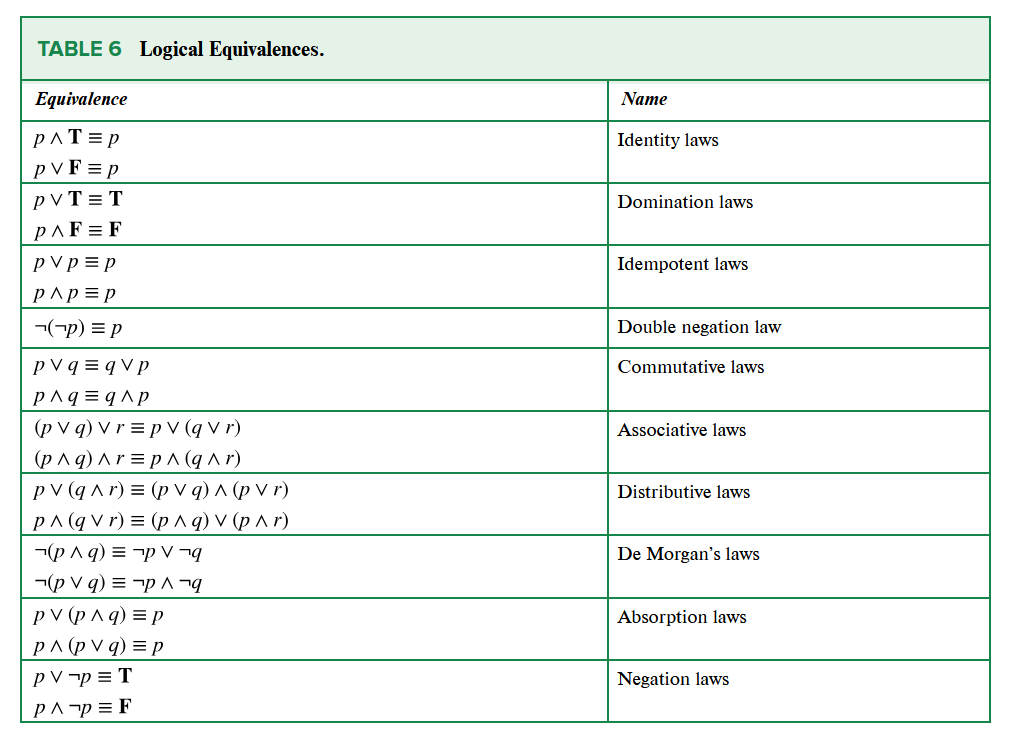
\includegraphics[width=0.72\textwidth]{1.3D.PNG}
    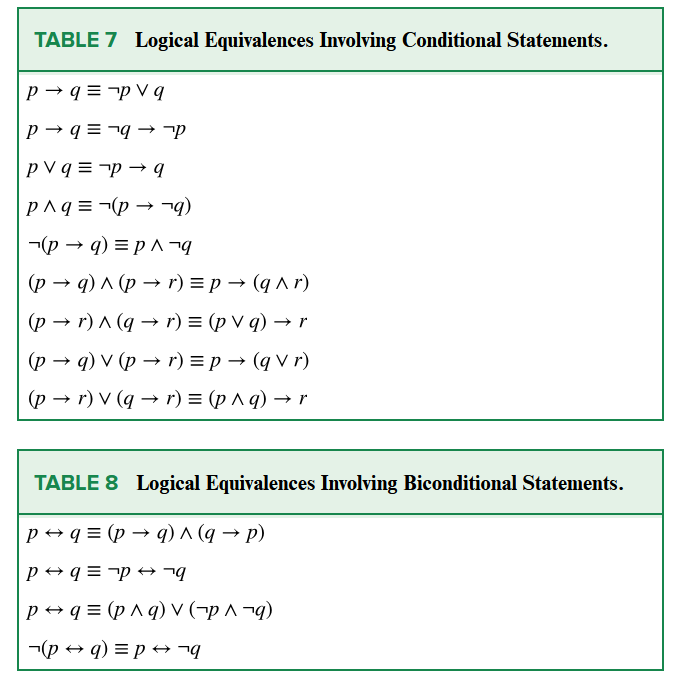
\includegraphics[width=0.72\textwidth]{1.3.D2.PNG}

\end{center}
Credit: Rosen's Discrete Mathematics 8e

When using De Morgan's Laws, remember to change the logical connective after you negate. 

De Morgan's Laws tell us how to negate conjunctions and how to negate disjunctions. The equivalence $\neg(p\lor q)\equiv \neg p \land \neg q$ tells us that the negation of a disjunction is formed from the conjunction of the negations of the component propositions. The negation of a conjunction also gives you the disjunction of the negations of component propositions.

A compound proposition is satisfiable if there is an assignment of truth values to its variables that make it true. If no such assignments exist, then it is unsatisfiable. 
\section{Predicates and Quantifiers}
We will introduce predicate logic now. For example in the statement $x$ is greater than 3, the variable is $x$ and the predicate is "is greater than 3".

In general a statement involving $n$ variables $x_1,x_2,\cdots,x_n$ can be denoted as $P(x_1,x_2,\cdots,x_n)$. 

\begin{definition}
    The universal quantification of $P(x)$ is the statement:
    \smallbreak
    "$P(x)$ for all values of $x$ in the domain."
    \smallbreak
    The notation $\forall x P(x)$ denotes the universal quantification of $P(x)$. Here $\forall$ is called the universal quantifier. An element for which $P(x)$ is false is called a counterexample to $\forall x P(x)$.
\end{definition}
\begin{definition}
    The existential quantification of $P(x)$ is the proposition:

    "There exists an element in $x$ in the domain such that $P(x)$"

    We use the notation $\exists x P(x)$ for the existential quantification of $P(x)$.
\end{definition}
Remember the truth value for both $\forall x P(x)$ and $\exists x P(x)$ depends on the domain.
\begin{center}
    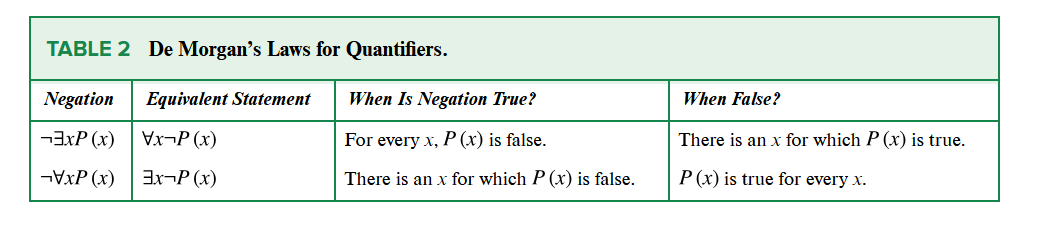
\includegraphics[width=0.9\textwidth]{1.4.PNG}
\end{center}
Credit: Rosen's Discrete Mathematics 8e

\section{Nested Quantifiers}
\section{Rules of Inference}
\section{Introduction to Proofs}
\section{Proof Methods and Strategy}

\end{document}